\chapter{}

\epigraph{"If 10 years from now, when you are doing something quick and dirty, you suddenly visualize that I am looking over your shoulders and say to yourself: 'Dijkstra would not have liked this', well that would be enough immortality for me."}{\textit{Edsger W. Dijkstra}}

\section*{The LEGv8 simulators landscape}

The current landscape of publicly available LEGv8 simulators can be divided into two categories: simulators that aim to reproduce the logical design presented in the textbook in chapter ?, and the simulators providing a high level simulation of the instruction set as defined in the book.
The survey was performed on GitHub using ``LEGv8'' and ``simulator'' as keywords and only those in a reasonably working state (as per the author) have been considered.

\subsection*{Software simulators}

\begin{table}[H]
	\centering
	\resizebox{\columnwidth}{40}{\small \begin{tabular}{|c|c|c|c|c|c|c|}
		\hline
		\textbf{Repository} & \textbf{Language} & \textbf{Integer Support} & \textbf{Pipelined} & \textbf{Registers view} & \textbf{Stack view} & \textbf{Floating Point Support} \\
		\hline
		\url{https://github.com/lcpckp/leg-cpu-sim} & Java & Partial & No & Yes & Yes & No \\
		\hline
		\url{https://github.com/chrwoods/legv8-emul} & C/C++ & Partial & Yes & Yes & Yes & No \\
		\hline
		\url{https://github.com/mtalyat/LEGv8Day} & C\# & Partial & No & Yes & Yes & No \\
		\hline
		\url{https://github.com/eaxworthy/LegV8Interpreter} & Python & Partial & No & Yes & Yes & No\\
		\hline
		\url{https://github.com/AdinAck/LEGv8-Simulator} & Swift & Partial & No & Yes & Yes & No \\
		\hline
		\url{https://github.com/anvitha305/legv8sim} & Python & Partial & No & Yes & Yes & Double precision only \\
		\hline
		\url{https://github.com/dangbandy/LegV8-Simulator} & C++ & Partial & No & Yes & Yes & No\\
		\hline
		\url{https://github.com/schang412/LEGv8-PyEmu} & Python & Partial & No & No & No & No\\
		\hline
		\url{https://github.com/GeorgePerreault/LEGV8_Interpreter} & Python & Partial & No & Yes & Yes & No\\
		\hline
	\end{tabular}}
	\caption{The surveyed software simulators}
\end{table}

They utilize high level languages such as C++, Python, Swift, TypeScript and Java. Some of them offer a graphical interface, pipelined execution and none of the implement the LEGv8 ISA in its entirety.



\subsection*{Hardware simulators}

\begin{table}[H]
	\centering
	\resizebox{\columnwidth}{45}{\small \begin{tabular}{|c|c|c|c|c|c|c|}
		\hline
		\textbf{Repository} & \textbf{Language} & \textbf{Integer Support} & \textbf{Pipelined} & \textbf{Floating Point Support} \\
		\hline
		\url{https://github.com/nxbyte/ARM-LEGv8} & Verilog & Partial & Yes & No \\
		\hline
		\url{https://github.com/phillbush/legv8} & Verilog & Partial & Yes & No \\
		\hline
		\url{https://github.com/ronitrex/ARMLEG} & Verilog & Partial & Yes & No \\
		\hline
		\url{https://github.com/mattco98/LEGv8-Processor} & Verilog & Partial & Yes & Partial \\
		\hline
		\url{https://github.com/amaurilopez90/LEGv8-CPU} & Verilog & Partial & Yes & No \\
		\hline
		\url{https://github.com/miguelangelo78/LEGv8-ISA} & Verilog & Partial & Yes & No \\
		\hline
		\url{https://github.com/brianworts/LEGv8_SingleCycle_Processor} & Verilog & Partial & Yes & No \\
		\hline
		\url{https://github.com/egflo/LEGv8} & Verilog & Partial & Yes & No \\
		\hline
		\url{https://github.com/ad153153/LegV8} & Verilog & Partial & Yes & No \\
		\hline
	\end{tabular}}
	\caption{The surveyed hardware simulators}
\end{table}

They use mostly Verilog as their hardware description language and implement an incomplete subset of the LEGv8 ISA. Some of them follow closely the design of the textbook while others expand upon it adding more executable instructions. None of them offer a graphical interface nor implement the ISA in its entirety.

\section*{ARM's LEGv8 simulator}

This is the simulator officially provided by ARM Education and is the subject of this thesis' work. It is written in Java 8 and uses Google's GWT framework to transpile the code into native JavaScript to allow the simulator to be executed inside a web browser as a normal web application. It provides a comprehensive user interface displaying an interactive text editor (provided by AceGWT) to input LEGv8 code and to display errors, and a visualization of the state of the \emph{X} registers.
When selecting the single-cycle execution mode, a visualizaton of the logical scheme of the LEGv8 ISA is presented and for each step of the execution various components change color to indicate the current stage of the pipeline. For the pipelined execution mode, the visualization is slightly modified to include pipeline-specific information such as pipeline registers, the hazard detection unit and the forwarding unit. An additional textual representation of the pipeline is provided to see the stage occupied by each instruction at any given moment.

\begin{figure}[H]
	\centering
	\subfigure[Single cycle]{
		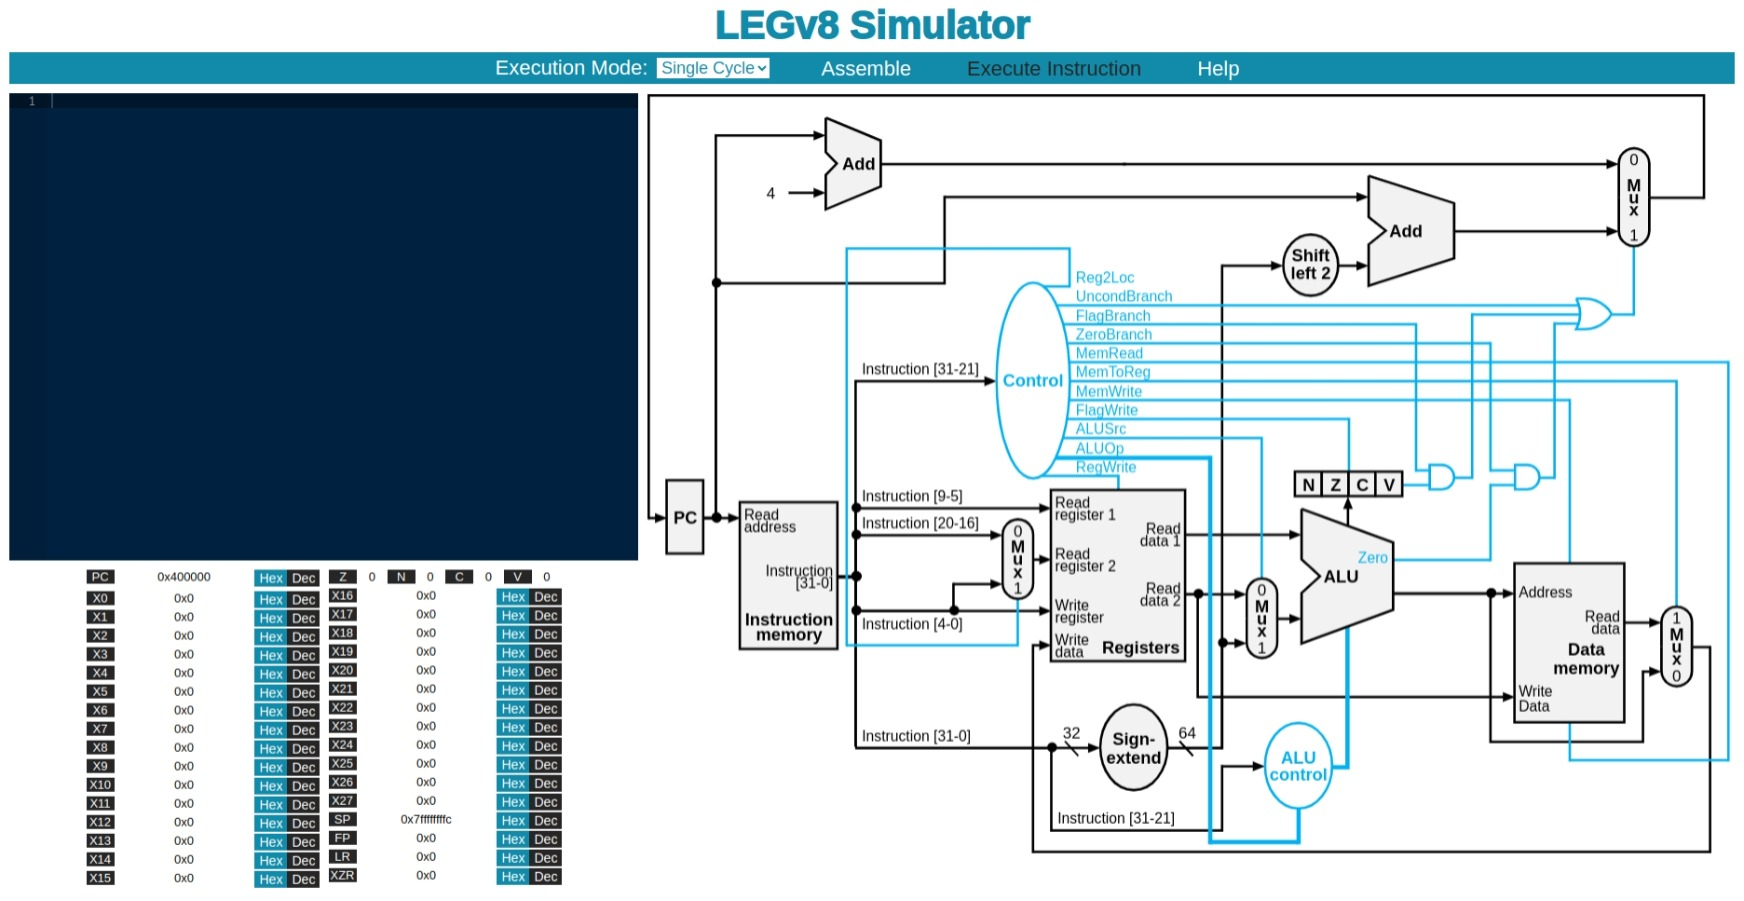
\includegraphics[width=.85\textwidth]{img/old_single_cycle.jpeg}
	}
	
	\subfigure[Pipeline]{
		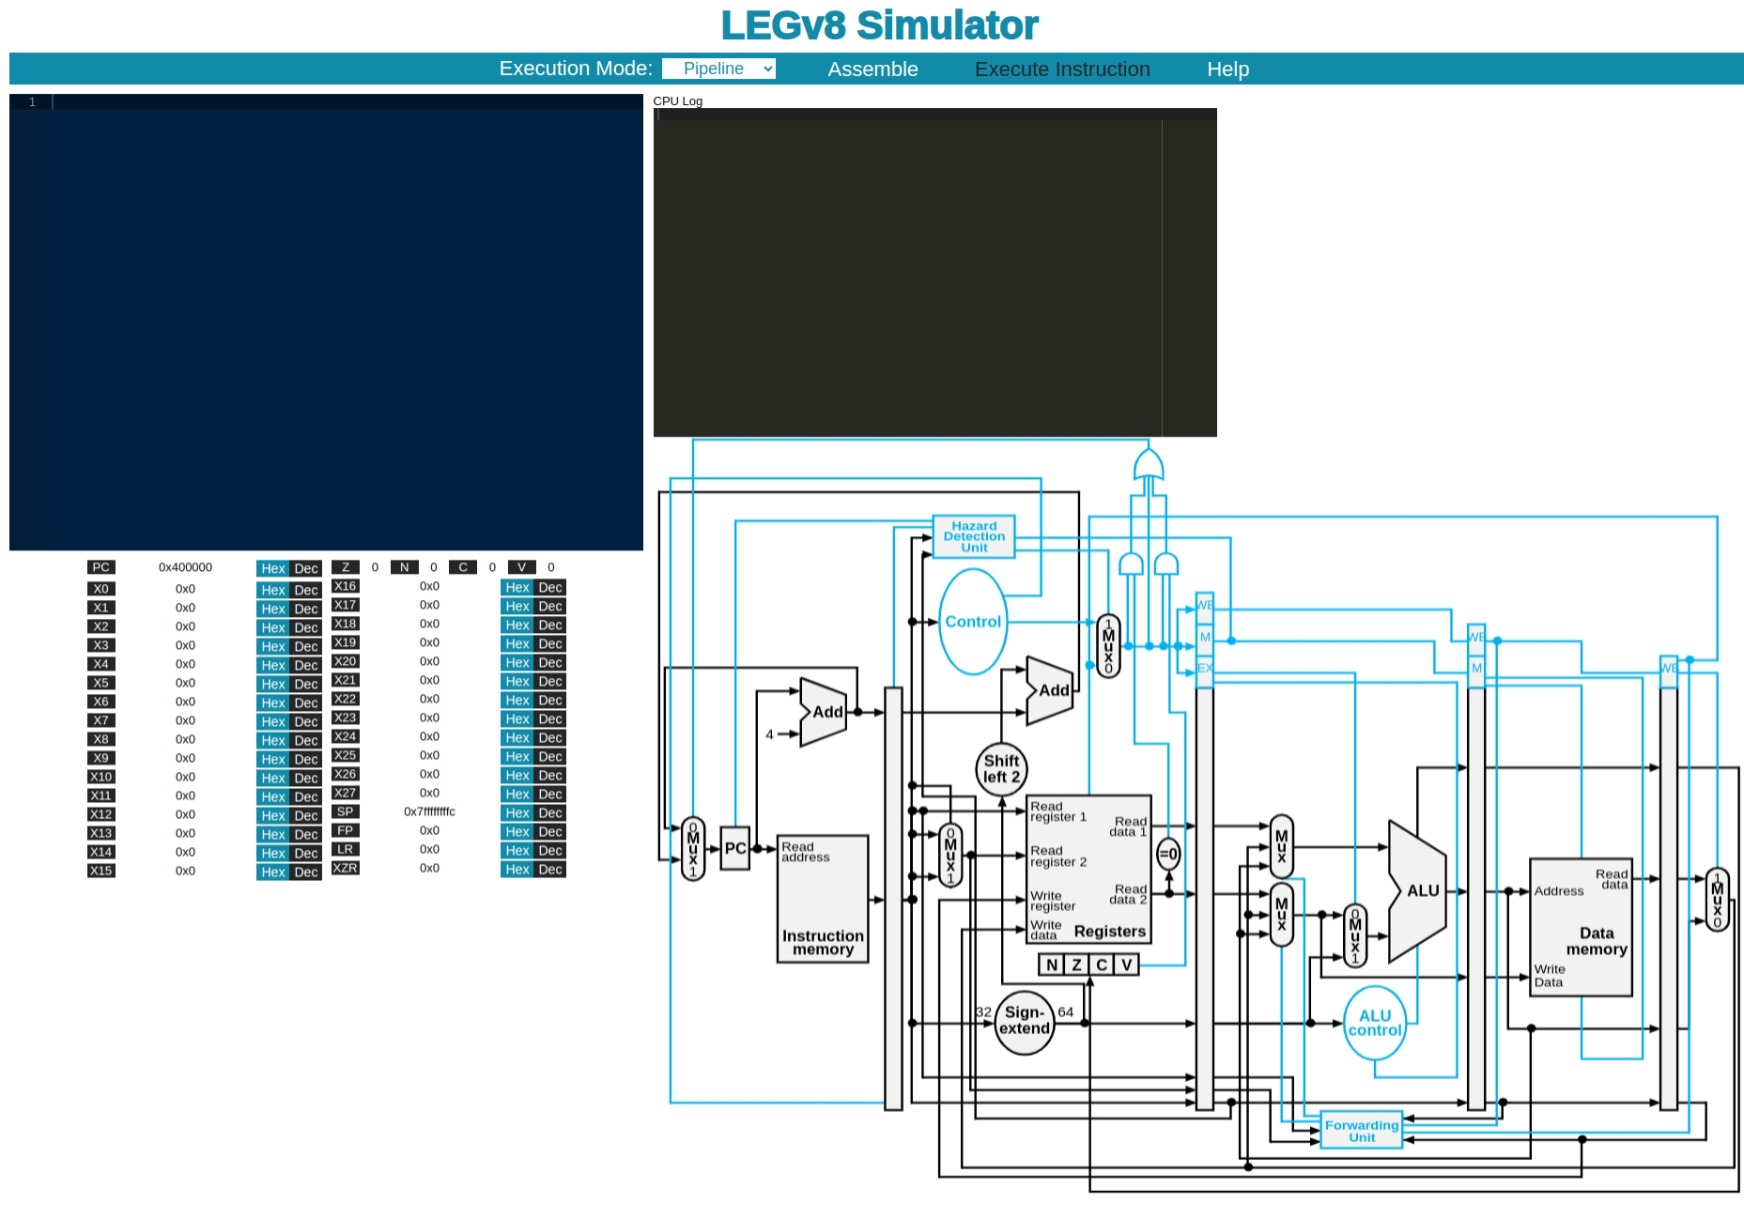
\includegraphics[width=.85\textwidth]{img/old_pipeline.jpeg}
	}
	\caption{The simulator's main page with the two different execution modes}
\end{figure}


Example of citations or references~\cite{einstein}\cite{latexcompanion}

\begin{figure}[h!]\label{fig:example}
\centering

\includegraphics[width=.8\textwidth]{img/units_logo.png}
\caption{Example of a figure}
\end{figure}

\lipsum[3]

\begin{figure}[!ht]
\centering
\subfigure[Subfigure 1]{
\includegraphics[width=.45\textwidth]{img/units_logo.png}}
\subfigure[Subfigure 2]{
\includegraphics[width=.45\textwidth]{img/units_logo.png}}
\subfigure[Subfigure 3]{
\includegraphics[width=.45\textwidth]{img/units_logo.png}}
\subfigure[Subfigure 4]{
\includegraphics[width=.45\textwidth]{img/units_logo.png}}
\caption{Example of figure with subfigures}
\label{fig:subexample}
\end{figure}

\lipsum[4]

\section{Dolor}
\lipsum[3]

\begin{table}
\centering
\begin{tabular}{|c|c|}
\hline
\textbf{Lorem} & \textbf{Ipsum} \\
\hline
\hline
Dolor & Sit \\
\hline
Amet &  \\
\hline
\end{tabular}
\caption{Example of a table}
\label{tab:example}
\end{table}

\lipsum[4-5]